\chapter{Benutzerzentrierte Auswertung} %TODO
Das folgende Kapitel erklärt das Konzept der Anforderungserhebung und Auswertung der graphisch-interaktiven Entwicklungsumgebung. Zu Beginn wird das Konzept des Fragebogens erläutert, mit dem die Anforderungen der Nutzenden erhoben wurden. Daraufhin wird die Struktur der Teilnehmenden Beobachtung aufgeführt mit dem das Feedback der Nutzenden gesammelt wurde, dies wurde unter anderem für die iterative Entwicklung, siehe Kapitel \ref{sec:iterative-entwicklung}, genutzt. Zu Ende des Kapitels wird die Anwendung dieser beiden Konzepte und die Rekrutierung der Nutzenden dargelegt. %TODO Das mit Ref?

%Das folgende Kapitel führt zunächst in die mögliche Bestimmung der Anforderungen der Nutzenden an eine graphisch-interaktive Entwicklungsumgebung ein. Daraufhin wird ein Konzept erläutert, wie eine solche Anwendung mit Hilfe von Nutzertests bewertet und verbessert werden kann. Zu Ende des Kapitels wird erläutert wie diese Konzepte umgesetzt und gezielt an die Zielgruppe verteilt wurden.

\section{Gestaltung der Anforderungserhebung} 
% Wie wurden anfänglich die Anforderungen der Nutzer erhoben? Wie wurden die Nutzer ausgewählt?

Um die Entwicklungsumgebung auf die Bedürfnisse der Nutzenden anzupassen, müssen anfänglich deren Anforderungen abgefragt werden. Zu diesem Zweck bietet sich, besonders durch die Möglichkeit der Einbindung von zusätzlichen Medien, eine gezielte Online-Befragung an \cite{Schnell2018MethodenES}. Aus den Ergebnissen dieser Befragung entstanden dann ein anfänglicher Style-Guide für die Benutzeroberfläche.

Damit die Befragung nützliche Ergebnisse liefert, müssen alle Fragen verständlich, knapp und neutral formuliert sein \cite{Jacobsen2019PraxisbuchUuU}. Der Fragebogen wurde in einzelne Abschnitte unterteilt, die alle nötigen Informationen enthielten und ohne Scrollen angezeigt werden konnten. Um technischen Problemen, die durch verschiedene Endgeräte und Browser entstehen könnten \cite{Schnell2018MethodenES}, vorzubeugen wurde die etablierte Online-Umfrage-Applikation LimeSurvey verwendet. 

Bevor Fragen den Teilnehmenden an der Umfrage Fragen gestellt wurden, wurde Pepper und das Anwendungsbeispiel in Abbildung \ref{fig:umfrage-anwendungsbeispiel} vorgestellt und erklärt. Im Folgenden werden die einzelnen Abschnitte und deren Nutzen für den Entwicklungsprozess aufgeführt. Die Auswertung der Ergebnisse des Fragebogens folgt in Kapitel \ref{sec:quanti-auswertung}.

\begin{figure}
	\centering
	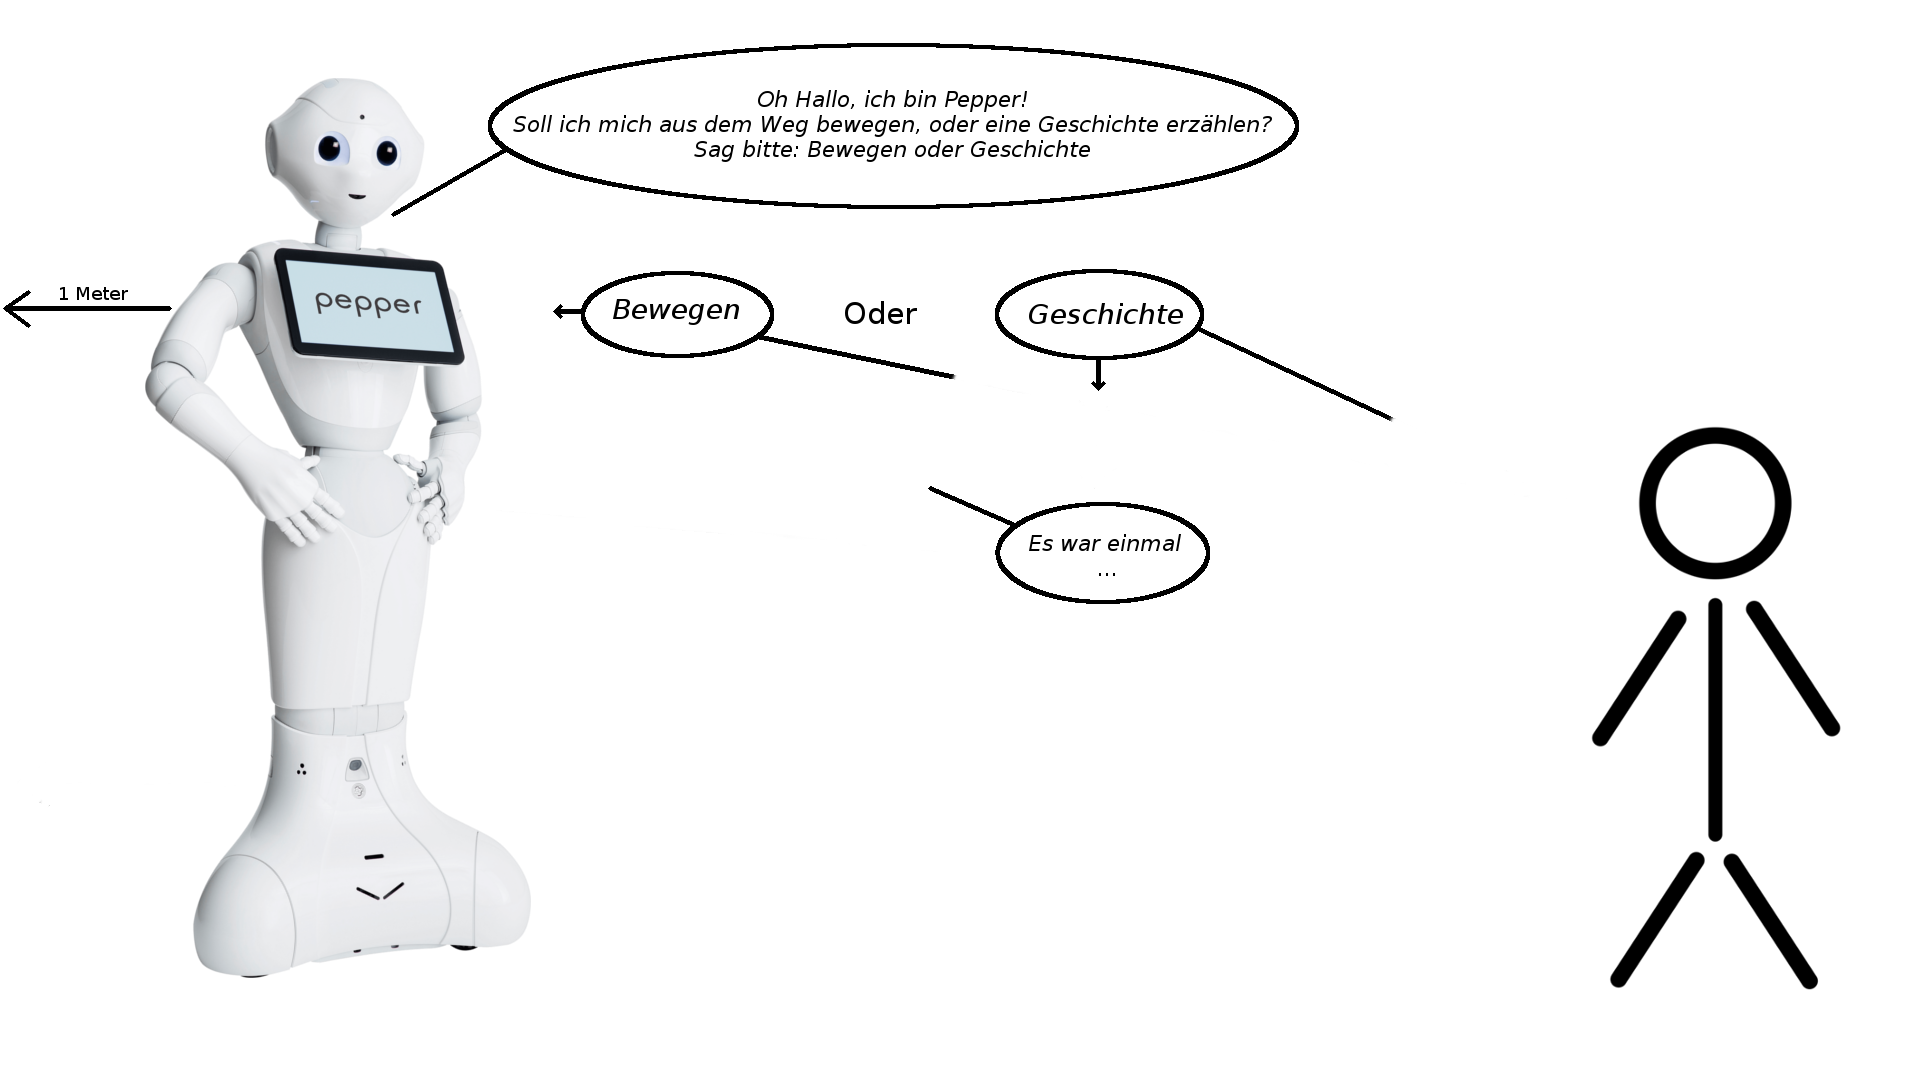
\includegraphics[width=13cm]{Plots/umfrage-anwendungsbeispiel.png}
	\caption{Anwendungsbeispiel der Anforderungserhebung.}
	\label{fig:umfrage-anwendungsbeispiel}
\end{figure}

%Damit die entstehende Entwicklungsumgebung genau auf die Bedürfnisse der Nutzer:innen angepasst ist, müssen anfänglich die Anforderungen der Nutzer abgefragt werden. Dazu bietet sich, besonders durch die Möglichkeit der Einbindung von zusätzlichen Medien, eine gezielte Online-Befragung an \cite{Schnell2018MethodenES}. Die Ergebnisse dieser Umfrage werden dann in einen Style-Guide für die Entwicklung der tatsächlichen Anwendung übersetzt.
%
%Neben Fragen zu Gestaltungsentscheidungen, wie die Platzierung von zusätzlichen Informationen oder der Eingabeform von Parametern, ist es auch nützlich die Anwendung mit etablierten Programmierumgebungen im Bezug auf die Greifbarkeit und Interesse an der Nutzung zu vergleichen. Des Weiteren können noch Anforderungen der Nutzer:innen an die Anwendung abgefragt werden, um die Relevanz von verschiedenen Funktionen für die Nutzer:innen zu vergleichen und diese entsprechend bei der Entwicklung der Prototypen zu priorisieren. Abschließend ist es hilfreich relevante demographische Informationen der Teilnehmer:innen abzufragen.
%
%Bei jeder der Fragen ist zu beachten, dass diese verständlich, knapp und neutral formuliert ist, sie nicht durch unnötige Verneinungen kompliziert werden, alle Teilnehmer:innen an der Umfrage die Frage beantworten können und ein Informationsgewinn durch die Beantwortung der Frage vorliegt \cite{Jacobsen2019PraxisbuchUuU}. Um technische Probleme zu vermeiden und die Umfrage möglichst barrierefrei auf verschiedensten Geräten und Browsern darstellen zu können, sollte eine Online-Umfrage-Applikation zu der Erstellung und Durchführung der Umfrage verwendet werden \cite{Schnell2018MethodenES}. Die verschiedenen Abschnitte des Fragebogens sollten jeweils auf einer eigenen Seite angezeigt werden, die ebenso den Fortschritt der Umfrage anzeigt. Diese einzelnen Seiten sollten alle nötigen Informationen beinhalten um die Fragen zu beantworten und ohne scrollen angezeigt werden können \cite{Jacobsen2019PraxisbuchUuU}.

\subsection{Vergleich mit bestehenden Anwendungen}
Im ersten Teil der Umfrage wird Choregraphe, siehe Kapitel \ref{sec:stand-der-technik}, und das in Kapitel \ref{sec:iterative-entwicklung} erläuterte Konzept der Entwicklungsumgebung mit Hilfe eines Mockups vorgestellt. Dabei werden die grundlegenden Funktionen beider Programme erläutert. Daraufhin wird jeweils die Implementierung des Anwendungsbeispiels aus Abbildung \ref{fig:umfrage-anwendungsbeispiel} in beiden Entwicklungsumgebungen angezeigt.

Die Teilnehmenden an der Umfrage werden aufgefordert mehrere Aussagen auf je einer 5-Punkte Likert-Skala für beide Entwicklungsumgebungen zu bewerten. Die Aussagen beziehen sich insbesondere auf Verständlichkeit der Benutzeroberfläche, Einschätzung der eigenen Fähigkeit die Entwicklungsumgebung zu nutzten und Interesse an der Nutzung der beiden Anwendungen. %TODO Direkt die Aussagen hier einbinden?

Die hier erhobenen Daten wurden dazu genutzt eine erste Einschätzung des Mockups zu erlangen und abzuwägen, ob ein direkter Vergleich der beiden Entwicklungsumgebungen zur Bewertung der entwickelten graphischen Oberfläche nötig ist.

%Ein Vergleich mit bestehenden Benutzeroberflächen ist nötig, um zu erfahren, ob der gewählte Ansatz einen Vorteil gegenüber bereits existierenden Lösungen darstellt. Besonders interessant ist ein Vergleich der Offenheit der Teilnehmer:innen an der Nutzung der verschiedenen Anwendungen.
%
%Um einen unbefangenen Vergleich zwischen den Ansätzen zu ermöglichen, wird erst eine Interaktions-Aufgabe eingeführt, die der Roboter ausführen soll. Im Folgenden werden sowohl die etablierte Software, als auch das erste Mock-Up der Entwicklungsumgebung vorgestellt und erklärt. Abschließend wird die Implementierung der anfänglich eingeführten Aufgabe in beiden Anwendungen abgebildet.
%
%Nach der Einführung in die Anwendungen werden mehrere Aussagen zu der Verständlichkeit und Interesse an der Nutzung einer solchen Benutzeroberfläche aufgeführt. Die Teilnehmer:innen an der Umfrage sollen dann ihre Übereinstimmung mit diesen Aussagen auf jeweils einer 5-Punkte Likert-Skala für alle vorgestellten Nutzeroberflächen beantworten. Abgefragte Einstellungen können Verständlichkeit der Benutzeroberfläche, Einschätzung der eigenen Fähigkeit die jeweilige Anwendung zu nutzen und weiteren Fragen zu spezifischen Teilen der Oberflächen beinhalten.
%
%Die aus diesen Fragen entstehenden Daten können zu einer Einschätzung führen, wie nützlich der gewählte Ansatz ist und ob eine weitere Verfolgung dieses Ansatzes hilfreich ist, oder ein andres Konzept ausgearbeitet werden muss.

\subsection{Blockgestaltung}
Wie bereits in Kapitel \ref{sec:visuelle-programmierung} dargelegt, gibt es verschiedene Möglichkeiten Blöcke in Blockly zu gestalten. Um diese Designentscheidungen den Nutzenden anzupassen, werden im zweiten Abschnitt der Online-Umfrage den Teilnehmenden jeweils verschiedene Mockups von funktional gleichen Blöcken präsentiert. Sie sollen dann den für sie am einfachsten verständlichen Block auswählen.

Die Auswahl der verschiedenen Optionen wurde so gewählt, dass die Mockups, die zur Auswahl stehen, jeweils Designentscheidungen repräsentieren. Beispielsweise steht die Entscheidung in Abbildung \textbf{TODO} repräsentativ für die Option einzelne Blöcke mit Hilfe von Drop-Down-Menüs zusammenzufassen und die Entscheidung Parameter-Slots generell extern (rechts) oder intern (mitten im Block) bereitzustellen. %TODO Zusammenschneiden der Designentscheidung 

Die gesammelten Antworten werden in den Style-Guide übersetzt, der die Vorlieben der Teilnehmenden an der Umfrage repräsentiert.

%Im darauf folgenden Abschnitt des Fragebogens werden verschiedene Funktionen des Roboters vorgestellt um Designentscheidungen am graphischen Interface der Entwicklungsumgebung zu treffen. Dazu werden jeweils mehrere Mock-Ups von Blöcken in Form von Bildern aufgeführt, die die beschriebene Funktion des Roboters umsetzen sollen. Die Teilnehmer:innen werden dazu aufgefordert, das Mock-Up auszuwählen, das am einfachsten zu verstehen ist. 
%
%Die Auswahl der Optionen ist so zu treffen, dass die Ergebnisse jeweils Designentscheidungen repräsentieren. Beispielweise können die Optionen die Nutzung von Drop-Down-Menüs, Textfeldern oder anderweitiger Eingabe von Parametern unterscheiden. Die hier gesammelten Antworten werden in einen Style-Guide übersetzt, der die Vorlieben der Nutzer:innen repräsentiert.

\subsection{Funktionale Anforderungen}
Im darauf folgenden Abschnitt des Fragebogens werden konkrete Anforderungen abgefragt. Den Teilnehmenden werden verschiedene Aussagen präsentiert, die sie auf einer 5-Punkte Likert-Skala bewerten sollen. Da die Teilnehmenden bereits eine Einführung in die Entwicklungsumgebung erhalten haben und sie im vorangegangenen Abschnitt des Fragebogens verschiedene Mockups und Kontrollelemente kennengelernt haben, haben sie nun ein Verständnis der Benutzeroberfläche um diese Anforderungen zu bewerten. %TODO etwas schöner formulieren?

Die abgefragten Anforderungen bezogen sich auf Barrierefreiheit, Sprache der Benutzeroberfläche, integrierte Funktionen in der Oberfläche, Benutzungsweise der Entwicklungsumgebung und weitere Funktionen dieser.

Teile dieser Anforderungen, wie die Sprache und Benutzungsweise der Benutzeroberfläche, flossen ebenso in den Style-Guide, siehe \ref{app:style-guide}, ein. Weitere Teile dieser Ergebnisse, wie etwa die Aussagen zu Barrierefreiheit, Erklärungen und Funktionen in der Benutzeroberfläche, bildeten eine Prioritäten-Liste von Funktionen, die in diese Anwendung eingefügt werden können.

%Eine weitere wichtige Komponente des Fragebogens ist die Abfrage der Anforderungen, die die Nutzer:innen an die Anwendung haben. Da diese inzwischen eine Einführung in die Entwicklungsumgebungen erhalten haben und in den Fragen zu den Designentscheidungen mit möglichen Mock-Ups der Kontrollelemente vertraut gemacht wurden, können sie hier einzelne Anforderungen einschätzen.
%
%Dies wird ebenfalls in Form von Aussagen umgesetzt, die die Teilnehmer:innen mit einer 5-Punkte Likert-Skala beantworten. Die Aussagen sind jeweils als technische Anforderungen formuliert, die Nutzer:innen von solchen Anwendungen an diese stellen könnten. Beispielsweise kann abgefragt werden, in welcher Sprache die Steuerelemente angezeigt werden sollten, welche weiteren Funktionen in der Oberfläche integriert werden sollten und welche Anforderungen an die Ausführung der Anwendung gestellt werden.
%
%Diese Ergebnisse werden dann teilweise, je nach Art der Aussage, in den Style-Guide oder eine Prioritäten-Liste der Anforderungen eingearbeitet, die die Wichtigkeit der Funktionen für die Prototypen und das endgültige Produkt angibt.

\subsection{Sonstige Datenerhebung}
Im abschließenden Teil der Umfrage wurden noch demographische Informationen, wie Studiengang und Semester, erfasst. Ebenso wurde die Programmier-Erfahrung der Teilnehmenden einfachen Ja-Nein-Fragen abgefragt.

Um Teilnehmende für die Nutzertests an den entstehenden Prototypen zu rekrutieren, wurden diese auf der letzten Seite der Online-Befragung dazu Aufgefordert eine E-Mail Adresse anzugeben. Da diese dann auch mit den Daten der vorangegangenen Fragen verknüpft sind, kann auch die Teilmenge der Nutzenden, die an den Nutzertests teilgenommen haben, in Kapitel \ref{sec:quanti-auswertung} einzeln betrachtet werden.

%In einem abschließenden Teil können noch Fragen gestellt werden, die Informationen über die Erfahrungen der Teilnehmer:innen mit Programmierung erheben. Ebenso können für die weiterlaufende Entwicklung relevante demographische Informationen abgefragt werden. Diese Abfrage kann in freier Form passieren.
%
%Um Teilnehmer:innen für die darauf folgenden Nutzertests an den entstehenden Prototypen zu rekrutieren werden diese auf der letzten Seite der Umfrage dazu aufgefordert bei Interesse ihre E-Mail Adresse anzugeben. Da diese dann auch mit den Daten der vorherigen Seiten verknüpft sind, kann später analysiert werden, ob die Teilnehmenden an den Nutzertests repräsentativ für die Befragten stehen.

\section{Instanziierung der Testsettings} %TODO
Wie wurden die entstandenen Prototypen getestet? Welche Aufgaben sollten die Nutzer durchführen? Welche Involvierung hatte der Beobachter der Tests?

\section{Operationalisierung}
Welche Nutzer? 